\chapter{Fundamente teoretice și tehnologii utilizate}

\section{Considerații generale}

Înainte de a descrie implementarea concretă, este utilă clarificarea fundamentelor pe care se sprijină proiectul. Favigon nu reunește doar câteva ecrane și endpoint-uri, ci mai multe idei care trebuie să funcționeze împreună: aplicație single-page, API REST, autentificare pe bază de token, persistare relațională, orchestrare containerizată, generare asistată cu ieșiri structurate și conversie dintr-un model intermediar către cod executabil.

Aceste noțiuni sunt tratate împreună deoarece în proiect ele nu apar izolat. De exemplu, editorul canvas este implementat pe frontend, dar depinde direct de modul în care proiectele sunt persistate în backend. Pipeline-ul AI produce o structură intermediară, dar valoarea ei reală se vede abia când motorul de conversie o transformă în fișiere HTML, React sau Angular. Din acest motiv, capitolul de față urmărește să explice nu doar \textit{ce} tehnologii sunt folosite, ci și \textit{de ce} alegerea lor a fost potrivită pentru problema rezolvată.

\section{Aplicații single-page și rolul frontend-ului modern}

Favigon folosește pe partea de client o aplicație Angular 20 organizată sub forma unui SPA. Într-un SPA, browserul încarcă inițial o singură pagină, iar apoi navigarea între ecrane este gestionată în principal client-side, fără reîncărcarea completă a documentului \cite{angularRouting2026}. Acest model este potrivit pentru Favigon din două motive.

Primul motiv este experiența utilizatorului. Editorul canvas presupune interacțiuni dese, actualizări vizuale rapide și trecere fluidă între zone precum profil, explore, settings, proiect și preview. Dacă fiecare navigare ar depinde de reîncărcarea integrală a paginii, aplicația ar deveni mai greu de folosit și mai puțin apropiată de instrumentele moderne de design.

Al doilea motiv este organizarea tehnică. Angular oferă rutare, componente, injecție de dependențe, gestiune a formularelor și integrare cu HTTP într-un ecosistem unitar. În plus, proiectul folosește componente standalone și `provideRouter`, ceea ce simplifică structura aplicației și reduce dependența de module tradiționale \cite{angularProvideRouter2026,angularStandalone2026}. Pentru un proiect în care cea mai mare complexitate se află în interfață, această coerență a framework-ului a contat mult.

Un element important în implementare este folosirea \textit{signals}. Documentația Angular prezintă signals ca mecanism reactiv granular pentru urmărirea și actualizarea stării \cite{angularSignals2026}. În editorul canvas, această abordare este utilă deoarece permite reacții mai fine la schimbarea selecției, a viewport-ului, a paginii curente sau a istoricului, fără a introduce un strat extern de management al stării. Pentru un feature foarte interactiv, această soluție oferă un raport bun între simplitate și control.

\section{Arhitectura client-server și API-ul REST}

Comunicarea dintre frontend și backend este organizată sub forma unui API REST. În literatura clasică, stilul REST este tratat ca o modalitate de proiectare a sistemelor software bazate pe resurse, interacțiuni standardizate și separarea clară între client și server \cite{fielding2000rest}. În Favigon, această alegere a fost una pragmatică.

Aplicația are resurse destul de clar delimitate: utilizatori, proiecte, design-uri, upload-uri, rezultate generate, relații sociale și operații de autentificare. Pentru fiecare dintre acestea a fost naturală definirea unor controllere și endpoint-uri specializate. Spre exemplu, proiectele sunt gestionate prin endpoint-uri dedicate pentru creare, actualizare, design, thumbnail, assets, like, star sau fork, în timp ce autentificarea este separată în propriul controller.

ASP.NET Core 9 a fost ales pentru backend deoarece oferă un cadru potrivit pentru API-uri moderne: rutare declarativă, middleware configurabil, DI integrat, autentificare, autorizare și extensibilitate la nivel de pipeline HTTP. Dincolo de faptul că framework-ul este matur, el permite și o separare curată între straturile aplicației. În proiect, API-ul doar primește cereri și returnează răspunsuri, în timp ce logica de business este ținută în servicii de aplicație, iar persistența și integrarea externă sunt mutate în infrastructură.

\section{Autentificare, token-uri și securitate la nivel de cerere}

Zona de autentificare din Favigon combină mai multe mecanisme: login și register clasic, OAuth cu furnizori externi, refresh token și autentificare în doi pași. Din perspectiva acestei lucrări, important este modul în care ele sunt integrate coerent.

ASP.NET Core oferă suport direct pentru autentificare JWT bearer \cite{aspnetJwt2025}. În proiect, token-ul de acces este transportat prin cookie HTTP only, iar backend-ul îl extrage din cookie-ul `jwt` în cadrul configurării `JwtBearer`. Practic, acest lucru combină avantajul token-ului auto-conținut cu avantajul unui transport mai greu de accesat din JavaScript. Această alegere nu elimină orice risc posibil, dar este rezonabilă pentru tipul de aplicație construit aici.

În plus, proiectul folosește refresh token separat și limitează calea cookie-ului de refresh la endpoint-ul de reînnoire, ceea ce reduce suprafața de expunere. Pentru operații sensibile sau scenarii de risc mai mare, este introdusă și autentificare în doi pași pe bază de cod temporar transmis prin email. Din perspectiva ghidurilor OWASP, folosirea unui factor suplimentar este una dintre cele mai eficiente măsuri pentru reducerea atacurilor care pornesc de la compromiterea parolei \cite{owaspAuth2026,owaspMfa2026}.

Dincolo de autentificare, backend-ul folosește și rate limiting. Documentația ASP.NET Core tratează rate limiting-ul ca mecanism de control al fluxului de cereri, util pentru protecție împotriva abuzului și pentru stabilitate \cite{aspnetRateLimiting2025}. În proiect sunt definite politici diferite pentru zone precum autentificare, AI, converter și users, tocmai pentru că profilul de risc și costul operațiilor nu sunt aceleași.

\section{Reprezentarea intermediară a interfeței}

Una dintre ideile de bază ale proiectului este că designul nu trebuie legat direct nici de canvas, nici de HTML final. Între aceste două niveluri este introdusă o reprezentare intermediară bazată pe noduri (`IRNode`), layout, stil, poziționare, metadate și variante responsive. Din punct de vedere conceptual, această reprezentare joacă rolul unui limbaj intern al aplicației.

Avantajul principal al unui astfel de model este separarea preocupărilor. Editorul poate să manipuleze elemente și structuri fără să producă imediat cod pentru browser. În același timp, motorul de conversie poate genera HTML, React sau Angular fără să depindă de detaliile de implementare ale editorului. Asta înseamnă că aceeași structură poate fi folosită în două scopuri diferite: editare și export.

În plus, modelul intermediar permite validare înainte de generare. Dacă un arbore de noduri este incomplet, inconsistent sau imposibil de randat corect, problema poate fi detectată înainte de etapa de export. Acesta este un avantaj important față de abordările care merg direct din prompt în cod. În Favigon, această validare intermediară face posibilă combinarea AI-ului cu un flux tehnic controlabil.

\section{JSON Schema și ieșiri structurate pentru AI}

În momentul în care s-a decis folosirea unui model AI pentru generarea interfețelor, una dintre primele probleme a fost fiabilitatea formatului de ieșire. Un răspuns foarte bun ca limbaj natural nu este automat util pentru o aplicație software. Este nevoie de date structurate, de câmpuri verificabile și de o formă care să poată fi procesată programatic.

Pentru această nevoie, JSON Schema este un instrument foarte potrivit. Specificația definește un mod standardizat de a exprima structura, tipurile și restricțiile unui document JSON \cite{jsonSchemaCore2022,jsonSchemaValidation2022}. În Favigon, schema este folosită pentru a constrânge ieșirile modelului AI atunci când se generează atât blueprint-ul intenției, cât și arborele intermediar al interfeței.

Din perspectiva OpenAI API, această idee este compatibilă cu \textit{structured outputs}, adică solicitarea unui răspuns care respectă o anumită schemă \cite{openaiStructuredOutputs2026,openaiChatCompletions2026}. Totuși, faptul că formatul este corect nu garantează automat că și conținutul este potrivit. De aceea, în implementare nu s-a mers doar până la schema JSON, ci au fost adăugate și validări semantice, plus un mecanism de reparare atunci când modelul produce ieșiri invalide sau incomplete.

\section{Baza de date relațională și persistența}

Pentru persistență este folosit PostgreSQL, prin Entity Framework Core și providerul Npgsql \cite{postgresql16docs2026,npgsqlEfCore2026}. Alegerea unei baze de date relaționale a fost firească, deoarece datele principale au relații clare: un utilizator poate avea mai multe proiecte, proiectele pot avea aprecieri și bookmark-uri, utilizatorii se pot urmări între ei, iar un proiect poate fi fork-uit din alt proiect.

Pe lângă modelul relațional clasic, aplicația păstrează și un câmp de tip JSON serializat pentru designul proiectului. Aici există un compromis asumat. Pe de o parte, datele vizuale ale canvas-ului sunt prea flexibile pentru a fi modelate comod în tabele relaționale fine. Pe de altă parte, utilizatorii, relațiile sociale și metadatele proiectelor se potrivesc foarte bine într-un model relațional. În practică, combinația dintre tabele relaționale și document JSON pentru design s-a dovedit suficient de echilibrată pentru scopul proiectului.

În implementarea concretă, schema rezultată este compactă, dar suficient de expresivă pentru produsul construit. Baza de date conține tabelele \texttt{users}, \texttt{projects}, \texttt{linked\_accounts}, \texttt{user\_follows}, \texttt{project\_bookmarks} și \texttt{project\_likes}. Tabelele relaționale descriu identitatea utilizatorului, proiectele, relațiile sociale și interacțiunile dintre utilizatori și proiecte, iar câmpul \texttt{DesignJson} din \texttt{projects} păstrează documentul de canvas sub formă \texttt{jsonb}. Această alegere permite filtrare și agregare eficientă pentru metadate, fără a forța fragmentarea structurii vizuale în numeroase tabele auxiliare.

Schema fizică include și constrângeri relevante pentru consistență. Email-ul utilizatorului este unic, conturile OAuth au unicitate atât pe perechea `(Provider, ProviderUserId)`, cât și pe perechea `(UserId, Provider)`, iar tabelele de tip follow, bookmark și like folosesc chei compuse pentru a preveni dublurile. În plus, proiectele folosesc o autoreferință prin `ForkedFromProjectId`, ceea ce face posibilă trasabilitatea unui fork fără a duplica separat noțiunea de proiect-sursă. Contextul EF Core completează automat timestamp-urile `CreatedAt` și `UpdatedAt`, astfel încât persistența să rămână coerentă și la nivel operațional, nu doar la nivel de structură.

\section{Orchestrare și infrastructură}

La nivel de infrastructură, proiectul folosește Docker Compose pentru definirea și pornirea serviciilor principale: baza de date PostgreSQL, API-ul, frontend-ul și tunelul Cloudflare \cite{dockerCompose2026,dockerComposeFile2026}. Această variantă reduce efortul necesar pentru pornirea locală și descrie într-un singur fișier dependențele dintre servicii, volumele persistente și rețeaua internă.

Avantajul principal al acestui mod de lucru este repetabilitatea. Când toate componentele importante sunt definite declarativ, mediul devine mai ușor de refăcut, de demonstrat și de mutat între sisteme. Pentru o lucrare de licență, acest aspect nu este deloc minor, deoarece ușurează demo-ul și reduce riscul ca aplicația să funcționeze doar pe o singură configurație locală.

În configurația actuală, fișierul \texttt{docker-compose.yml} nu pornește doar containerele, ci exprimă și câteva decizii operaționale utile. Baza de date are \textit{healthcheck}, astfel încât API-ul să nu pornească înainte ca PostgreSQL să fie pregătit pentru conexiuni. API-ul montează separat volumul pentru upload-uri, ceea ce permite persistența imaginilor și thumbnail-urilor independent de ciclul containerului. Frontend-ul este construit cu argument explicit pentru fișierul de mediu de producție, iar tunelul Cloudflare este atașat peste aplicația deja pornită, nu folosit ca substitut pentru rețeaua internă.

\begin{table}[H]
  \centering
  \caption{Servicii și volume definite în orchestrarea locală a proiectului}
  \label{tab:docker-servicii}
  \renewcommand{\arraystretch}{1.15}
  \begin{tabularx}{\textwidth}{>{\RaggedRight\arraybackslash}p{2.8cm}YY}
    \toprule
    \textbf{Serviciu / volum} & \textbf{Rol principal} & \textbf{Observații utile} \\
    \midrule
    \texttt{db} & instanță PostgreSQL 16 pentru persistența relațională & folosește \textit{healthcheck} cu \texttt{pg\_isready} și volum persistent dedicat \\
    \texttt{api} & aplicația ASP.NET Core expusă intern pe portul 8080 & depinde de sănătatea bazei de date și montează directorul de upload-uri \\
    \texttt{frontend} & aplicația Angular compilată pentru mediu de producție & depinde de API și rulează în aceeași rețea internă \\
    \texttt{cloudflared} & publicare externă controlată prin Cloudflare Tunnel & folosește token extern și pornește doar după frontend \\
    postgres data & persistă datele PostgreSQL & evită pierderea datelor la recrearea containerelor \\
    uploads data & persistă fișierele încărcate și thumbnail-urile & separă conținutul generat de ciclul de build/deploy \\
    \bottomrule
  \end{tabularx}
\end{table}

Pentru expunerea aplicației în exterior este folosit și Cloudflare Tunnel. Documentația oficială subliniază faptul că tunelul funcționează prin conexiuni doar outbound dintre infrastructura locală și rețeaua Cloudflare, evitând expunerea directă a unui IP public și reducând suprafața de atac \cite{cloudflareTunnel2026}. În proiect, această alegere a fost utilă mai ales pentru publicare și testare externă, fără a complica prea mult configurarea rețelei. Vederea simplificată a stack-ului rezultat este redată în Figura~\ref{fig:stack-favigon}.

\begin{figure}[H]
  \centering
  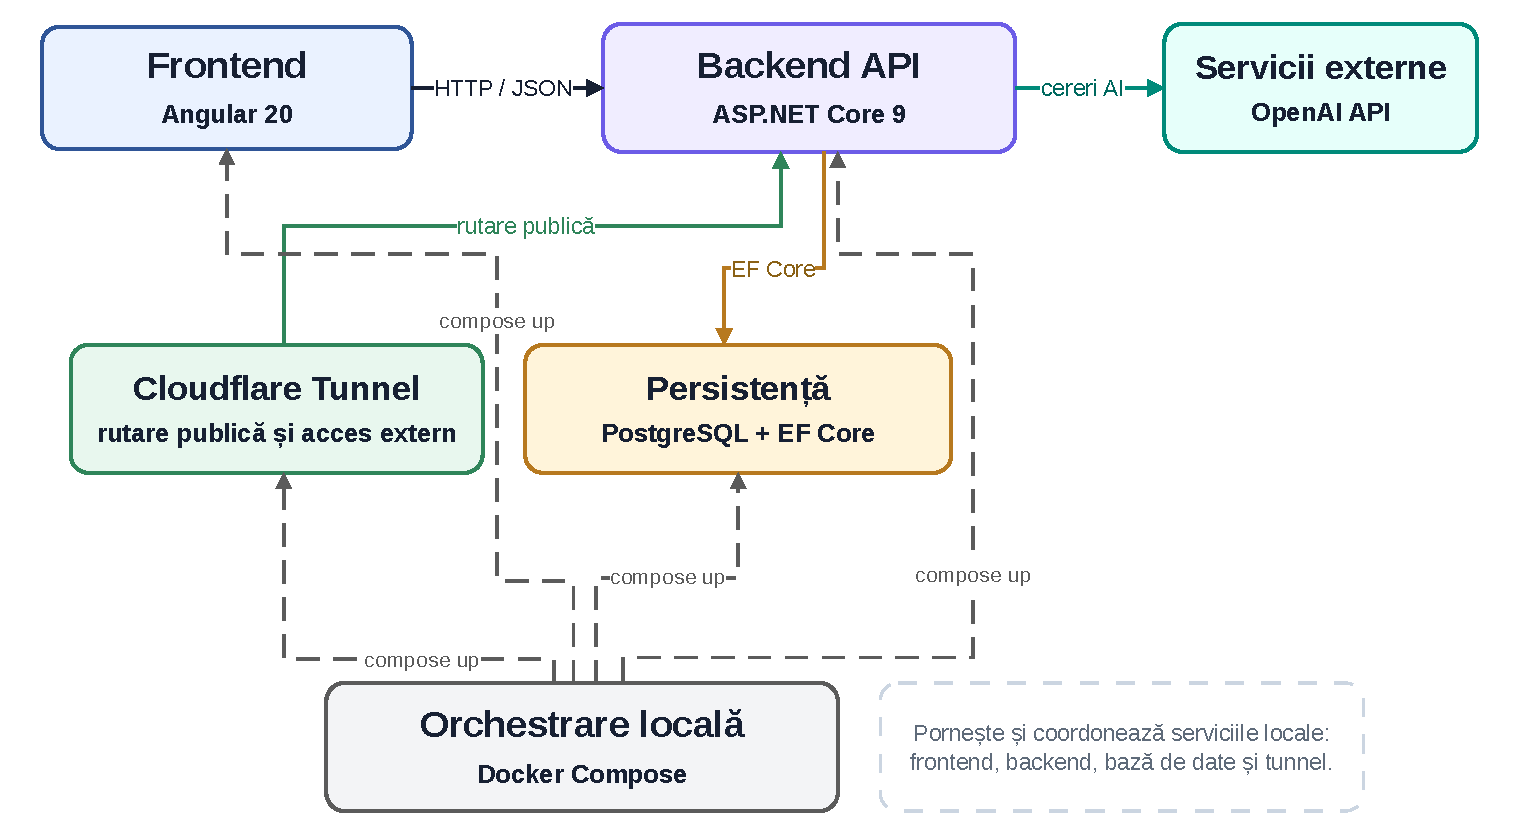
\includegraphics[width=\textwidth]{diagrams/stack-favigon.drawio.pdf}
  \caption{Vedere simplificată asupra stack-ului tehnologic folosit de Favigon}
  \label{fig:stack-favigon}
\end{figure}

\section{De ce această combinație tehnologică a fost potrivită}

Privită în ansamblu, combinația Angular + ASP.NET Core + PostgreSQL + OpenAI API + Docker Compose nu este una neobișnuită. Tocmai aici stă avantajul ei practic. Sunt folosite tehnologii bine documentate, mature și suficient de separate ca responsabilitate. Angular acoperă interfața și interacțiunea clientului. ASP.NET Core acoperă API-ul și middleware-ul. PostgreSQL acoperă persistența relațională. OpenAI API acoperă generarea asistată. Docker Compose și Cloudflare Tunnel simplifică operaționalizarea.

Această alegere are și un beneficiu pedagogic. Într-o lucrare de licență, prea multe tehnologii neobișnuite riscă să mute accentul de pe soluția inginerească pe complexitatea setării mediului. Aici valoarea nu vine din folosirea unor instrumente rare, ci din modul în care acestea sunt combinate pentru a obține un produs coerent.

\section{Concluzii intermediare}

Fundamentele prezentate în acest capitol explică de ce Favigon a fost construit în forma actuală. SPA-ul susține interacțiunea rapidă. API-ul REST și separarea pe straturi susțin claritatea backend-ului. JWT-ul, 2FA și rate limiting-ul susțin securitatea operațională. Reprezentarea intermediară și JSON Schema susțin controlul asupra generării AI și a exportului. PostgreSQL și Docker Compose susțin stabilitatea și portabilitatea.

Pe baza acestor fundamente, capitolul următor trece la analiza și proiectarea sistemului propriu-zis: cerințe, actori, fluxuri, model de date și arhitectură internă.


